We gebruiken bovenstaande code om \math{sin(x)} en $\frac{1}{(1+7*x^2)}$ te benaderen op het interval [-2,2] met een equidistante set van 9 absciswaarden. We vergelijken dit ook met een veelterminterpolant door deze punten. Het resultaat is te vinden in figuur \ref{fig:sinequi}. TODO verdere uitleg over verschil veelterm vs. spline.

\begin{figure}
\centering
\begin{subfigure}{.5\textwidth}
  \centering
  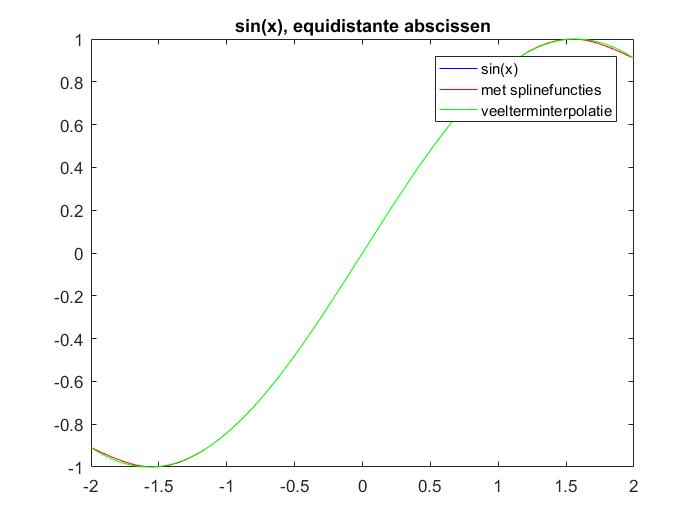
\includegraphics[width=.4\linewidth]{afbeeldingen/sin_equi.jpg}
  \caption{functiewaarden}
\end{subfigure}%
\begin{subfigure}{.5\textwidth}
  \centering
  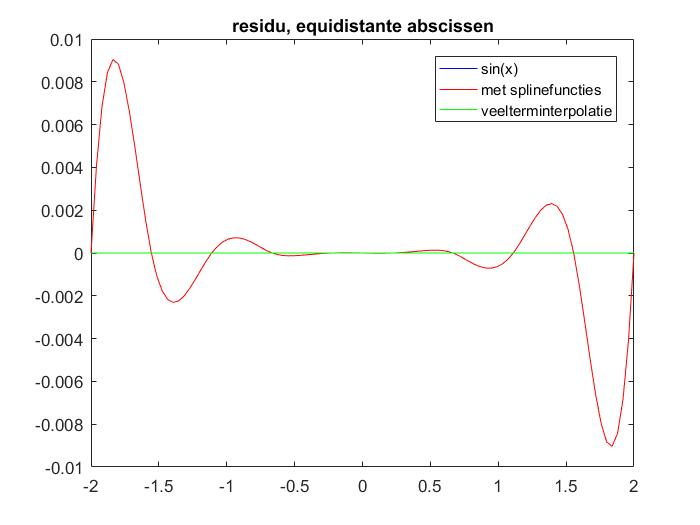
\includegraphics[width=.4\linewidth]{afbeeldingen/sin_equi_res.jpg}
  \caption{residu}
\end{subfigure}
\caption{interpolant door 9 absciswaarden van \math{sin(x)}}
\label{fig:sinequi}
\end{figure}

TODO figuren rationale functie invoegen
TODO figuren groter maken, juist schikken